%!TEX root = ../template.tex
%%%%%%%%%%%%%%%%%%%%%%%%%%%%%%%%%%%%%%%%%%%%%%%%%%%%%%%%%%%%%%%%%%%%
%% chapter4.tex
%% NOVA thesis document file
%%
%% Chapter with lots of dummy text
%%%%%%%%%%%%%%%%%%%%%%%%%%%%%%%%%%%%%%%%%%%%%%%%%%%%%%%%%%%%%%%%%%%%

\typeout{NT FILE chapter4.tex}%

\chapter{Proposal}
\label{cha:proposal}

This section will define all aspects our microservice contract evolution approach.
The adaptation approach, the service registry and benchmark platforms will all be defined.

\section{Scope} % (fold)
\label{sec:scope}

The proposed solution will only support HTTP contracts, because
most applications require a web presence and
microservice teams prefer to use a single protocol for both internal and external communications.

Other event-driven and request-response protocols, such as RPC,
have simplified contracts, and there are already a number of tools that support the evolution of schemas for these protocols,
albeit with some limitations.

\section{Adaptation Approach} % (fold)
\label{sec:adaptation_approach}

The adaptation approach was already introduced, now we will give a more detailed description.

The evolution of contracts is supported by lightweight proxy's capable of dynamically adapting messages exchanged between services to match them with the static service code.
To support this mechanism we will need tree ingredients, a contract description language, a compatibility verification and adaptation protocol.

\paragraph{Contract Description Language}

Contracts in web services can be described with the use Web Api Description Languages (WADL).
The OpenAPI specification is the most widely adopted WADL for HTTP services, instead of designing yet another WADL,
we aim to extend the OpenAPI specification to incorporate support for the needs of our approach.

We will use the Json format to represent records in messages.
Json lacks a language for describing schemas, however, the OpenAPI specification supports the description of record schemas in conjunction with the signature of HTTP endpoints.

\paragraph{Compatibility Verification}

Two approaches will be presented for the verification of contracts:

- Approach A. In a simplified approach, the verification process determines whether a new version of a producer
is compatible with earlier versions that are being consumed, without analyzing the references of each endpoint.
If a new contract contains an endpoint that is incompatible with a previous version, all consumers of that version,
even if they do not use the incompatible endpoint, are unable to use the new version.
The advantage of this approach is that consumer references don't need to be described and documented;
the verification only processes the producer's new contract and its previous versions.
The disadvantage of this approach is that there are deployments that are deemed unsafe despite being safe.

\paragraph{}

- Approach B. In an alternative approach, the verification processes both the producer contract and all the consumer references in each endpoint for
assessing the safety of a deployment operation.
The advantage of this approach is that are no false negatives when accessing the safety of deployments.
The disadvantage is that developers will face an additional burden because consumer references will need to be documented.
One way to mitigate this disadvantage is to detect consumer references through the analysis of the system logs.

\paragraph{}

The compatibility of endpoints and references is typically accomplished via the comparison of element names.
Elements with the same name are considered to be the equal.
In this case, some ambiguous evolutions can only be solved with human intervention and knowledge of the domain.
For example: renaming two fields of the same type; inserting a new field and removing another of the same type, is indistinguishable from renaming a field.
To solve this problem without requiring human intervention,
all elements must be tagged with an immutable and unique key,
and the verification process must use element keys rather than element names.
Editors for low-code visual languages, such as OutSystems or Kony Mobility, can manage element keys transparently and automatically;
however, in the proposed approach, tags must be manually inserted in the WADL definitions.

\paragraph{}
In the case of solution A. the compatibility verification can be done with human intervention without imposing a significant burden
because it involves comparing only the active versions of one producer 1-$1^{\ast}$.

\paragraph{}
In the case of solution B. the compatibility verification needs to be fully automatic because it involves comparing a new version of a producer, with all consumers 1-N.

\paragraph{}

In Approach A. the verification process automatically outputs a compatibility file for each pair (N,O) where N is the new contract version,
and O is an earlier contract version that is still being consumed.
In this file all mappings between elements in each contract are explicitly defined.
This file can be audited by a developer before it is used in the adaptation protocol.
If the compatibility verification detects an ambiguous case, the developer is notified, and the system only continues after the ambiguity is resolved.

Approach A has an additional advantage over Approach B, in that it supports more complex evolution types, because it can be done with human intervention.
Unlike Approach B, which only supports the removal, addition,
and renaming of fields, Approach A. can accommodate complex changes,
such as changing the format of a date, through the use of user-defined adaption functions.

(eg. new\_contract.startdate = formatDate(earlier\_contract.startdate, format))

These functions can be defined in a static library or provided through mobile code.


To define this functions with mobile code, a compatibility specification would be produced in the verification process;

In proposed solution we are more inclined to investigate solution A. because it allows

To solve this problem for each pair of versions (new, old) a compatibility specification file is produced;

The system notifies the programmer if such a case occurs and request intervention for its resolution.


Each operation's signature in every contract can be expressed as a function.
For each pair of versions (new, old) a compatibility specification file is produced;

This file contains the associations between the old version function/parameter keys, and the new version parameters keys (eg. old:k0 -> new:k1; old:k1->new:k5);

This file is audited by a programmer before being used for the generation of the adapter proxy code
In case of incorrect mapping between parameter types the programmer can fix manually.







The compatibility verification functions in two steps:

At first stages

Intuitively, the compatibility verification checks if all the items replaced
by the modules in the system will be compatible to the ones effectively used by the
remaining services, and if the requirements of the new modules are satisfied by the
existing resources in the system.

chemas can then be checked based
on version identifiers and compatibility relations just like in our case [22].

his is a relation established by
a compile-time procedure and is a precondition for the deploy operation along with
other deploy-time verifications that we define at this point.

Our type system is parametric on
a signature-based compatibility relation on service contracts, and we foresee that it
can be extended to richer semantic contracts.

HTTP a contract includes the HTTP method, the path, the schema of the parameters, and the location of parameters (path, query, header).

\section{Service Registry} % (fold)
\label{sec:service_registry}

Each operation's signature in every contract can be expressed as a function.
For each pair of versions (new, old) a compatibility specification file is produced;

In this file all functions and parameters are associated with a key;

Records are expanded/exploded and each of its parameters is associated with a key, the record itself is also associated with a key;

This file contains the associations between the old version function/parameter keys, and the new version parameters keys (eg. old:k0 -> new:k1; old:k1->new:k5);

This file is audited by a programmer before being used for the generation of the adapter proxy code
In case of incorrect mapping between parameter types the programmer can fix manually.

Some ambiguous evolutions can only be solved with human intervention and knowledge of the domain;
The system notifies the programmer if such a case occurs and request intervention for its resolution.

Examples:
renaming two fields of the same type;
inserting a new field and removing another of the same type, is indistinguishable from renaming a field;

Default values can also be supplied inside compatibility specification in order to de-clutter service API or implementations;

More complex signature changes (such as the change of parameter unit from celsius to fahrenheit, the change of date format, the partition of name parameter into surname and first name)
can be accommodated in the combinability specification with the use of functions (eg. extractFirstName(old:k0) \textrightarrow new:k1  extractSurname(old:k0) \textrightarrow new:k1)

This functions can be made available through static libraries, or more interestingly, the programmer could write their implementation in the compatibility specification file
and afterwards they would be integrated in adapter proxy coded before compilation;

The versions of service API are collected in a schema registry;

When a new version is submitted for deployment the registry is consulted in order to obtain the set of all active versions of the same service;

\begin{figure}[htbp]
    \centering
    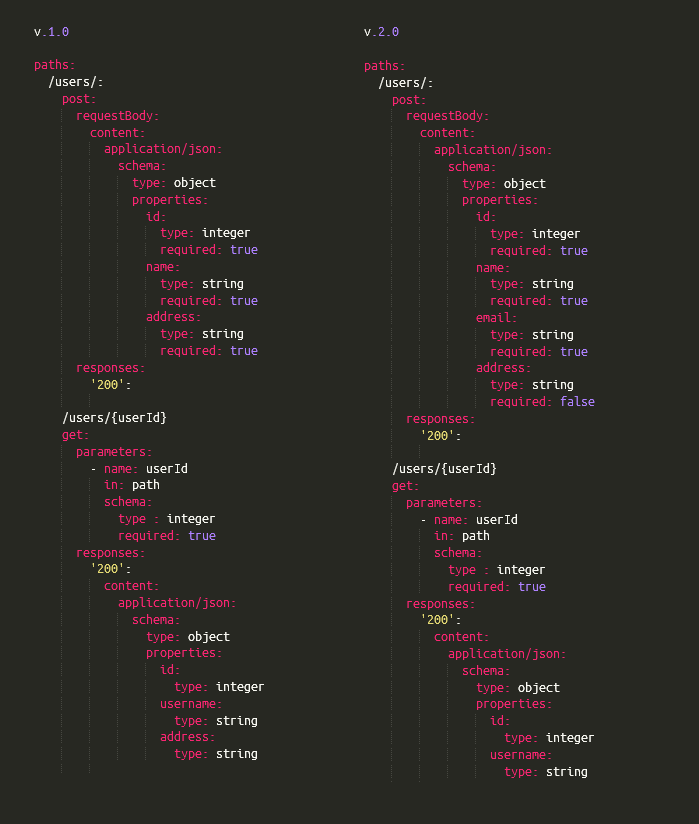
\includegraphics[height=5.7in]{simple_sig}
    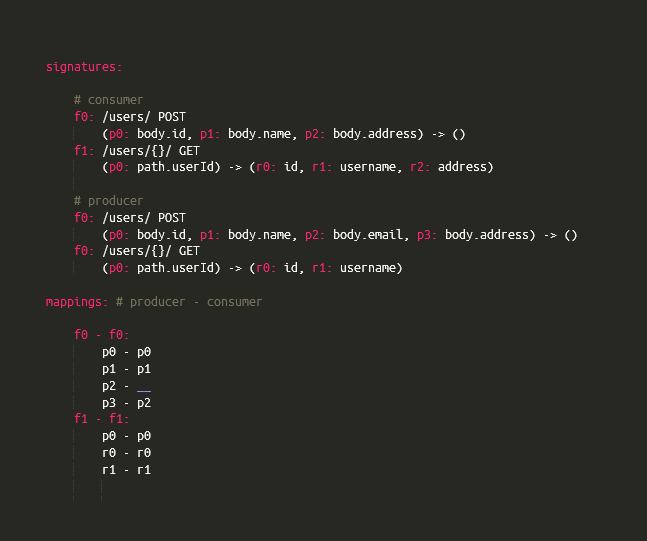
\includegraphics[height=4in]{map}
    \caption{Service contracts}
    \label{fig:simple}
\end{figure}

\section{Benchmark platform} % (fold)
\label{sec:benchmark_platform}

\begin{figure}[htbp]
    \centering
    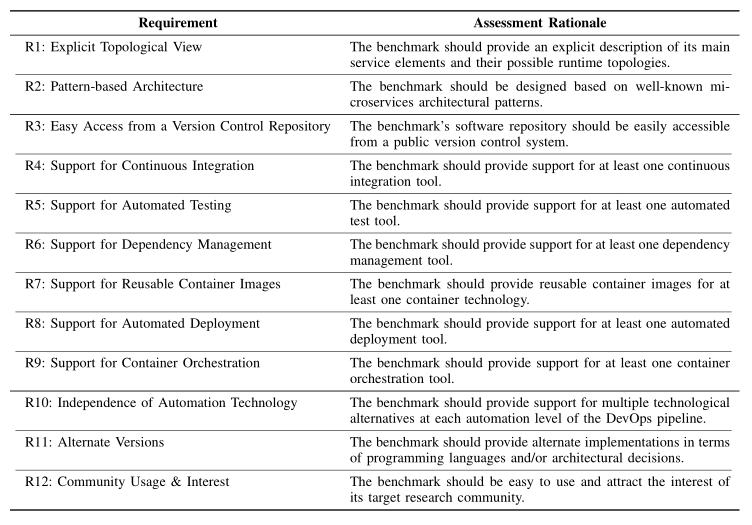
\includegraphics[height=4in]{benchmark_requirements}
    \caption{Benchmark Requirements}
    \label{fig:benchmark}
\end{figure}

The platform's main requirement is the ability to evaluate different solutions in comparable scenarios while utilizing the same evaluation criteria. It must also be capable of evaluating a solution without requiring modifications to an existing implementation.

Experiments must be simple to share and reproduce by different individuals.

It should be straightforward to aggregate reported metrics for a certain time period between two events, such as the beginning and conclusion of the evolution of a service.

The platform must allow users to specify how and when each service should evolve via a pipeline configuration file or directly through a terminal.

\paragraph{Approaches under assessment}

\paragraph{Rollover deployments}
A rolling deployment is a deployment strategy that slowly replaces previous versions of an application with new versions.
A new batch of instances is launched before taking the old instances out of service.

\paragraph{Data-serialization languages with schema evolution support }
Frameworks such as Protobuf, Thrift, and Avro offer data schema evolution, although their support is severely limited and lacks assurances about the safety of deployment operations.

\paragraph{Proxy Adapter}
A proxy is injected into a micro-service image, which intersects all requests and responses and modifies messages, allowing involved services to communicate without subscribing to the same contract version.

\paragraph{Benchmark platform architecture}

\begin{figure}[htbp]
    \centering
    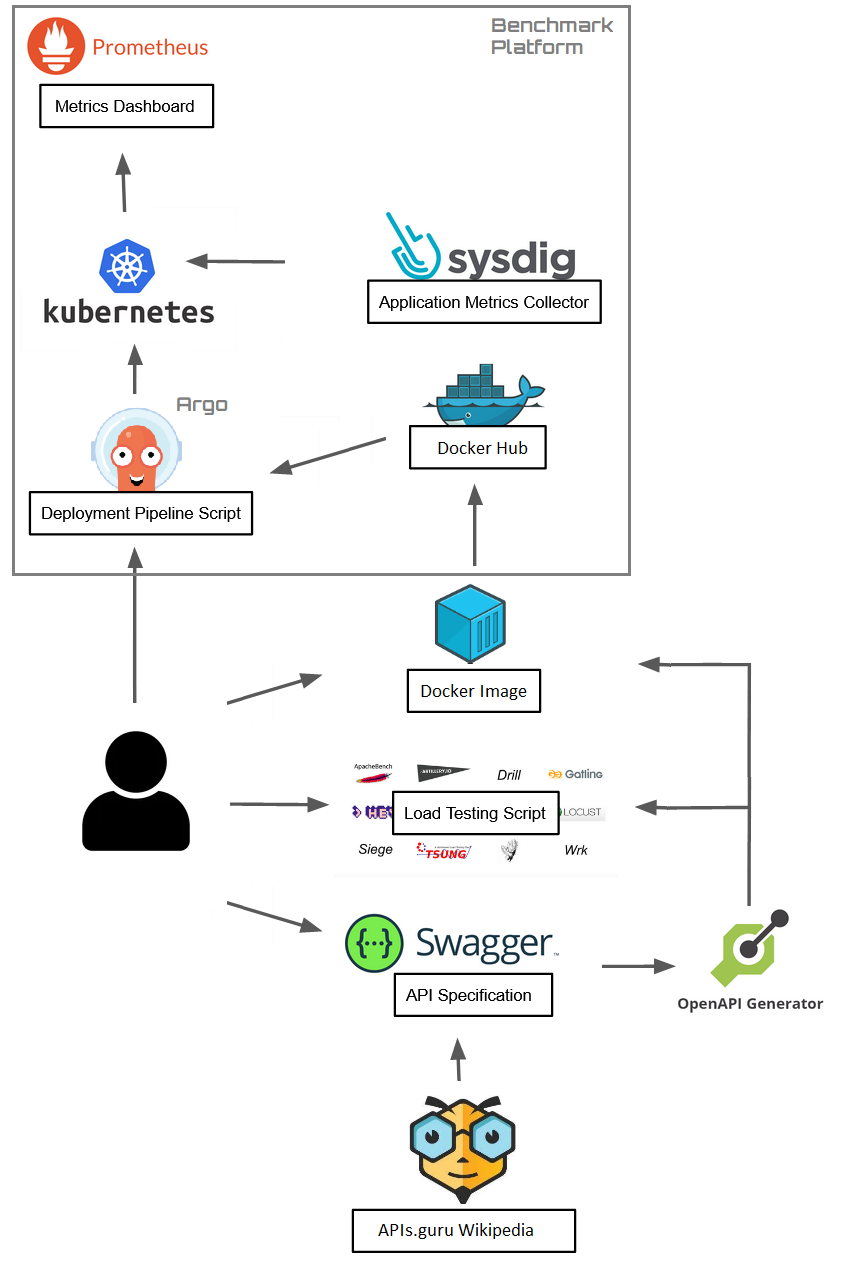
\includegraphics[height=3in]{canvas}
    \caption{The figure illustrates the benchmark platform components}
    \label{fig:canvas}
\end{figure}

\paragraph{Services evolution} can be specified in a Argo workflow through tasks.
Argo is a robust pipeline engine for Kubernetes, It provides simple, flexible mechanisms for specifying constraints between tasks and for linking the output of any task as an input to subsequent task.

Complex experiments can be made with Argo since the state of each deployment in Kubernetes can be queried via a task and utilized as input in a decision that leads to different tasks.

\paragraph{Active virtual users} The Argo workflow file may be used to specify how and when each service should evolve, as well as to manage active virtual users by deploying and stopping docker images that contain load testing scripts.


\paragraph{Test Implementations}
Developing implementations (for a specific evolution strategy) is a time-consuming endeavor because several versions of the same app are required to test its evolution.
API.guro contains the APIs for a few apps in various versions.
The open-AI generator project can produce bare-bones server implementations based on the swagger specification of a app.
The produced implementation does nothing by default; modifications would be required for services to be able to discover and communicate with one another.
It will be necessary to choose application APIs and develop each application service in several versions.

\paragraph{Results}
Metrics are collected via the kubernetes logging API that is accessed by Promotheus. Prometheus is a pull-based monitoring system. It periodically sends HTTP scrape requests, the response to this requests is parsed in storage along with the metrics for the scrape itself.
Kurbenetes does not gather application-specific metrics by default, such as latency and error rate. Sysdig monitor fixes this problem without needing application instrumentation by leveraging the eBPF protocol to obtain information about all system calls straight from the kernel.
With the conjunction of this tools is possible to evaluate the latency, error rate, traffic, and saturation of each service individually in an event-based time series.

Gathered data may be visualized in real-time using Grafana dashboards, that can be customized through Prometheus.
Prometheus provides a query language that allows metrics to be aggregated by events or components.
Raw data from Prometheus can also be downloaded.